\section{Methods}
\subsection{PCA for feature extraction}

PCA is an orthogonal transformation of data, converting a vector $\mathbf{x}$ of
a high-dimensional feature space into a vector $\mathbf{y}$ of a lower
dimensional space. It does so by constructing an orthogonal subspace whose basis
define directions which capture most of the given data's variance. The elements
of the transformed vector $\mathbf{y}$ form the set of linearly uncorrelated
variables called \textit{principal components}. 

Mathematically the PCA can be viewed as the statistical interpretation of the
singular value decomposition (SVD): Given a data matrix
$\mathbf{X}\in\mathbb{R}^{n\times m}$ a unique matrix decomposition exists:

\begin{equation}
  \mathbf{X} = \mathbf{U \Sigma V}^T,
\end{equation}

where $\mathbf{U}\in\mathbb{R}^{n\times n}$ and
$\mathbf{V}\in\mathbb{R}^{m\times m}$ are orthonormal matrices, and
$\mathbf{\Sigma}\in \mathbb{R}^{n\times m}$ contains the \textit{singular
values} $\sigma_i$ on its diagonal. Both $\mathbf{U}$ and $\mathbf{V}^T$
resemble an orthonormal basis for the column and row space of $\mathbf{X}$,
respectively. Assuming the columns of X comprise of data entries $\mathbf{x}$,
$\mathbf{U}$ forms the newly found basis.  

In PCA terminology, the columns of $\mathbf{U}$ are called \textit{principal
axis} while the already mentioned \textit{principal components} are obtained by
$\mathbf{U^Tx}$. The first principal axis represents the largest variance of the
data and is equal to the eigenvectors belonging to the largest eigenvalue of the
data's covariance matrix \footnotemark. The following columns represent the next
variances, all arranged in decreasing order with respect to eigenvalues of the
covariance matrix or the singular values of $\mathbf{X}$. Thus, the PCA
components, arranged in the order according to their decreasing variance,
represent the most important statistical information contained in the original
set of data. 

\footnotetext{Note that mathematically correct, the covariance matrix is defined
on the mean-subtracted or centered data matrix $\bar{\mathbf{X}}$}

\begin{figure}[ht]  
  \centering
  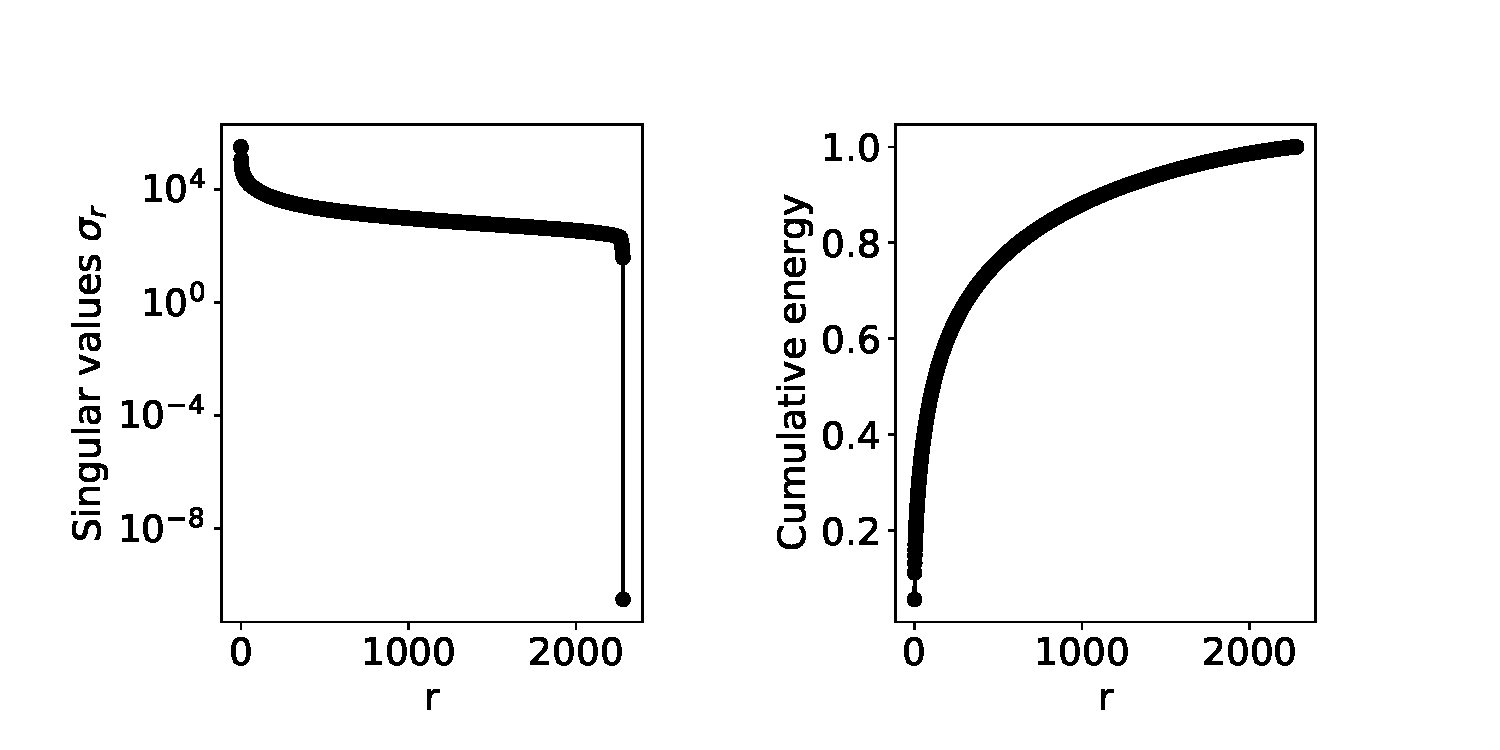
\includegraphics[width=\columnwidth]{singularValues.pdf}
  \caption{(left) Singular values $\sigma_k$ (right) Cumulative energy /
  variance captured by the first $r$ principal components in the Yale Face B
  Database}
  \label{sv}
\end{figure}

By limiting the number of principal components, which translates to truncating
$\mathbf{U}$ to $\tilde{\mathbf{U}}$, and keeping the most important
eigenvalues, one achieves dimensionality reduction. Given an orthogonal basis of
the so found subspace $\tilde{\mathbf{U}}$, an arbitrary vector can be projected
to the lower dimensional space by means of a projection matrix
$\mathbf{\tilde{U}\tilde{U}^T}$ denoted in Eq. (\ref{eq:projection}). As seen in
Fig. \ref{sv} it is possible to plot the singular values versus the number of
components. The amount of variance captured in the first $r$ modes is given by
Eq. (\ref{eq:energy}).

\begin{gather}
 \textrm{``Cumulative energy of data''} = \frac{\sum\limits_{k=1}^{r}{\sigma_k}}{\sum{\sigma_k}} \label{eq:energy} \\
 \mathbf{y = \tilde{U}\tilde{U}^Tx} \label{eq:projection}
\end{gather}

This gives a guideline on how many components to keep in order to capture a
certain amount of variance.

In the context of FR, the PCA or SVD decomposes the data into very intuitively
interpretable components. Applied to a large library of facial images, the
principal axis are the so called \textit{eigenfaces}. They are the basis of the
newly computed coordinate system with which one can reconstruct old or even
generate completely new faces, meaning every face image in the original set of
data can be represented as a linear combination of these eigenfaces. Fig
\ref{eigenfaces} shows some of those eigenfaces. In appendix Fig.
\ref{appendix:reconstruction} I have included an example where I tried to
reconstruct a new face image with the eigenfaces of the Yale Face B Database
\cite{yalefaceB}. 

\begin{figure}[ht]
  \centering
  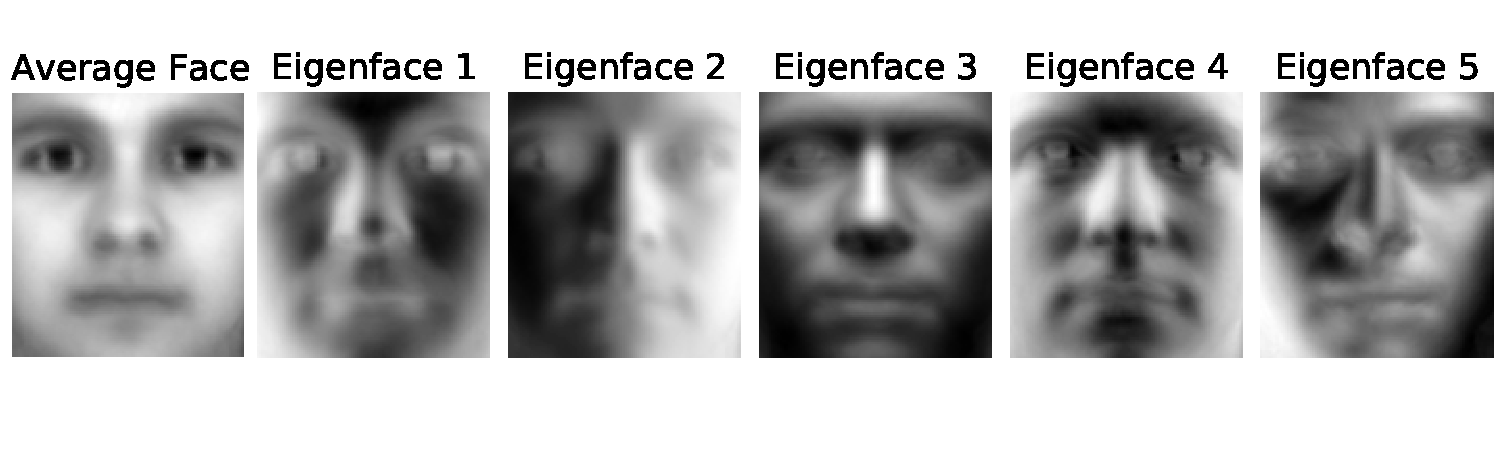
\includegraphics[width=\columnwidth]{eigenfaces.pdf}
  \caption{Average face and first five eigenfaces of the Yale Face Database B}
  \label{eigenfaces}
\end{figure}

Images of the same person tend to cluster in the eigenface space, making this a
useful tool for facial recognition and classification. A demonstration of PCA's
classification ability is shown in Fig. \ref{cluster}. For facial feature
extraction I will be using a chosen amount of principal components,
interpretable as the weights of the eigenfaces. These signals create the
patterns which are characteristic for the particular class/individual and
represent the coding of the image. They will serve as the input attributes to
the output classifier.

\begin{figure}[ht]
  \centering
  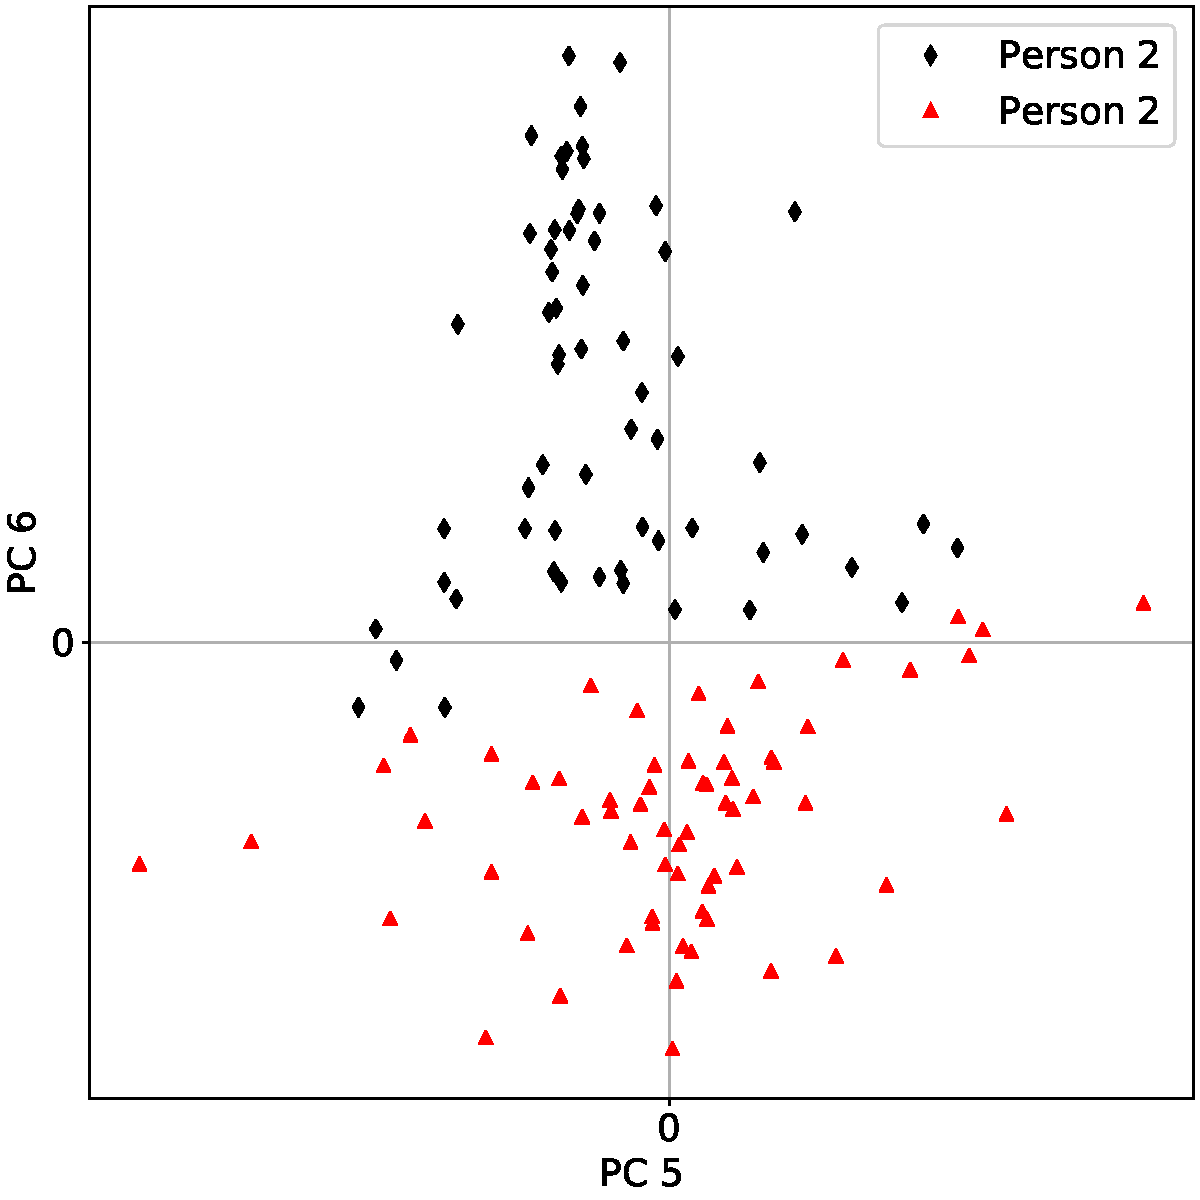
\includegraphics[width=0.7\columnwidth]{PCAcluster.pdf}
  \caption{Projection of all images from two individuals onto the 5th and 6th 
  PCA components}
  \label{cluster}
\end{figure}
